\section{Results}\label{sec:results}
\begin{itemize}
	\item discuss results per hypotheses
	\item \david{we could also put the methodology here and focus the last section on utterance embeddings?}
	\item ...
\end{itemize}

Utterance embeddings have the property of encapsulating the meaning of utterances from the words that compose them; as with the case of word embeddings, these representations present appealing relations from which similar words (in a semantic sense) appear close by in the high dimension space. We being by extracting samples from the SwDA corpus belonging to clear unrelated tags, and applying dimensionality reduction to their vector representations and plotting the results in 2 and 3 dimensions. The sampled utterances belong to the following categories: \emph{Wh-questions}, \emph{Thanking}, \emph{Reject}, and \emph{Apology}. Considering the words that are used in these kind of units, sample points should be clearly separated. The utterance embeddings were extracted using a 300-dimensional model trained on the SwDA corpus interjected with Google pretrained vectors. Figure~\ref{fig:2d_pca} and Figure~\ref{fig:3d_pca} show scatter diagrams of the utterance embeddings after applying PCA.

\begin{figure}
\centering
\begin{minipage}{.23\textwidth}
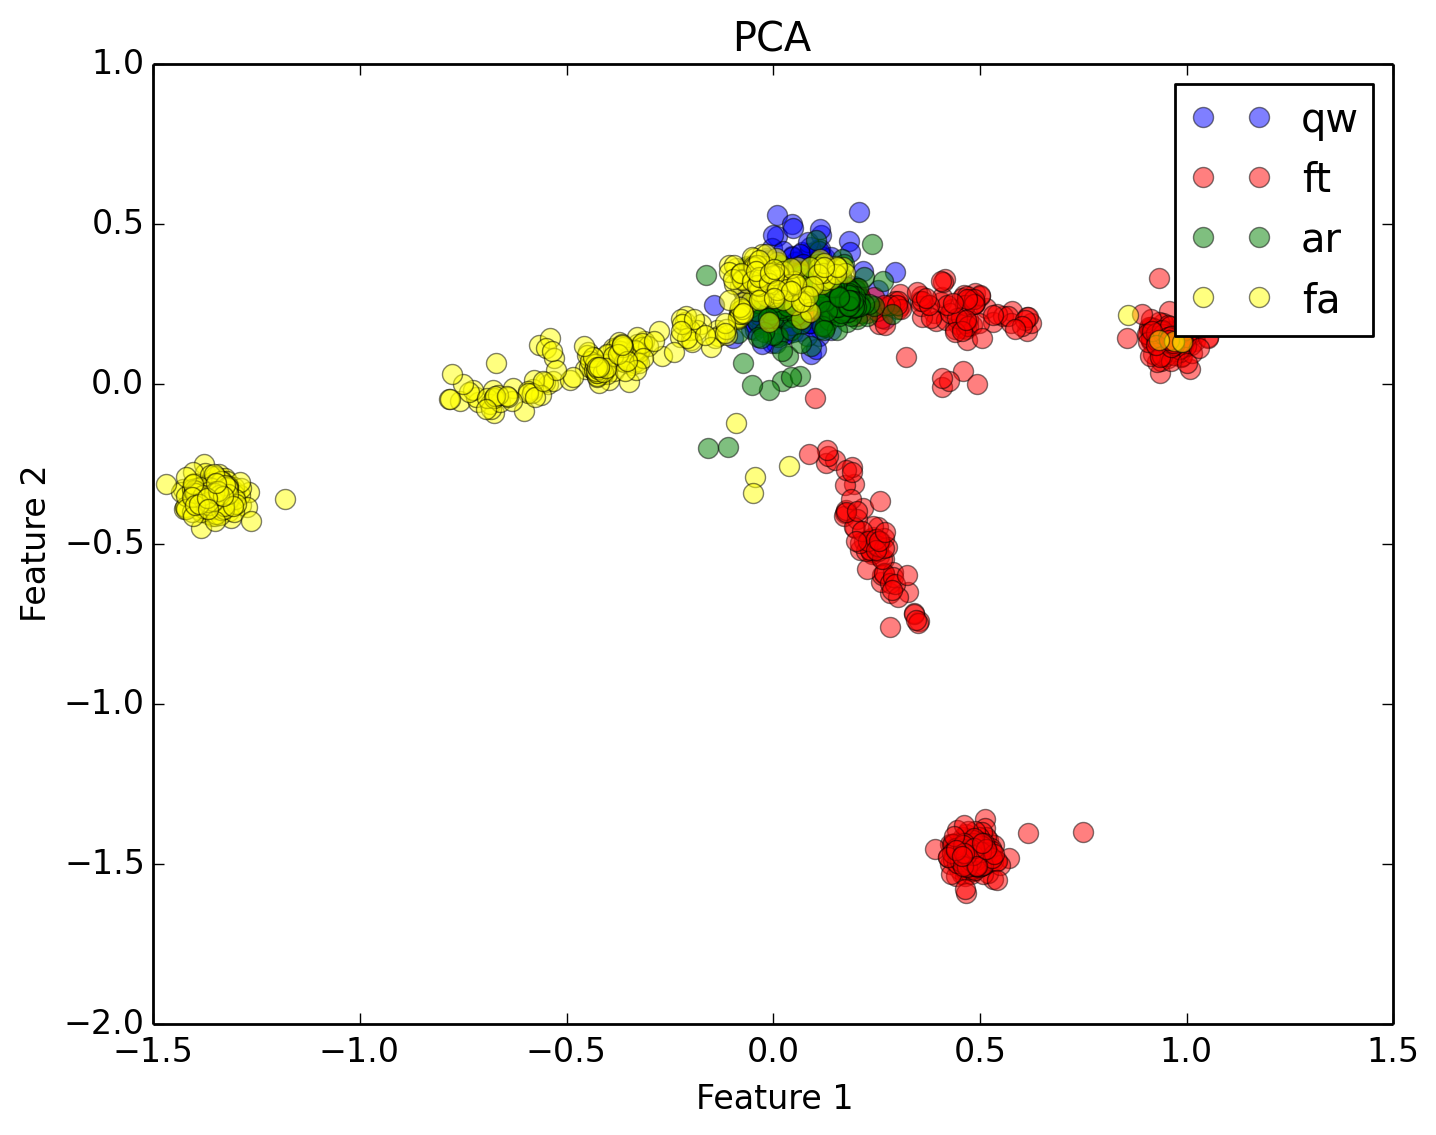
\includegraphics[width=1\textwidth]{img/easy_pca_2d}
\caption{2D PCA.}
\label{fig:2d_pca}
\end{minipage}
\begin{minipage}{.23\textwidth}
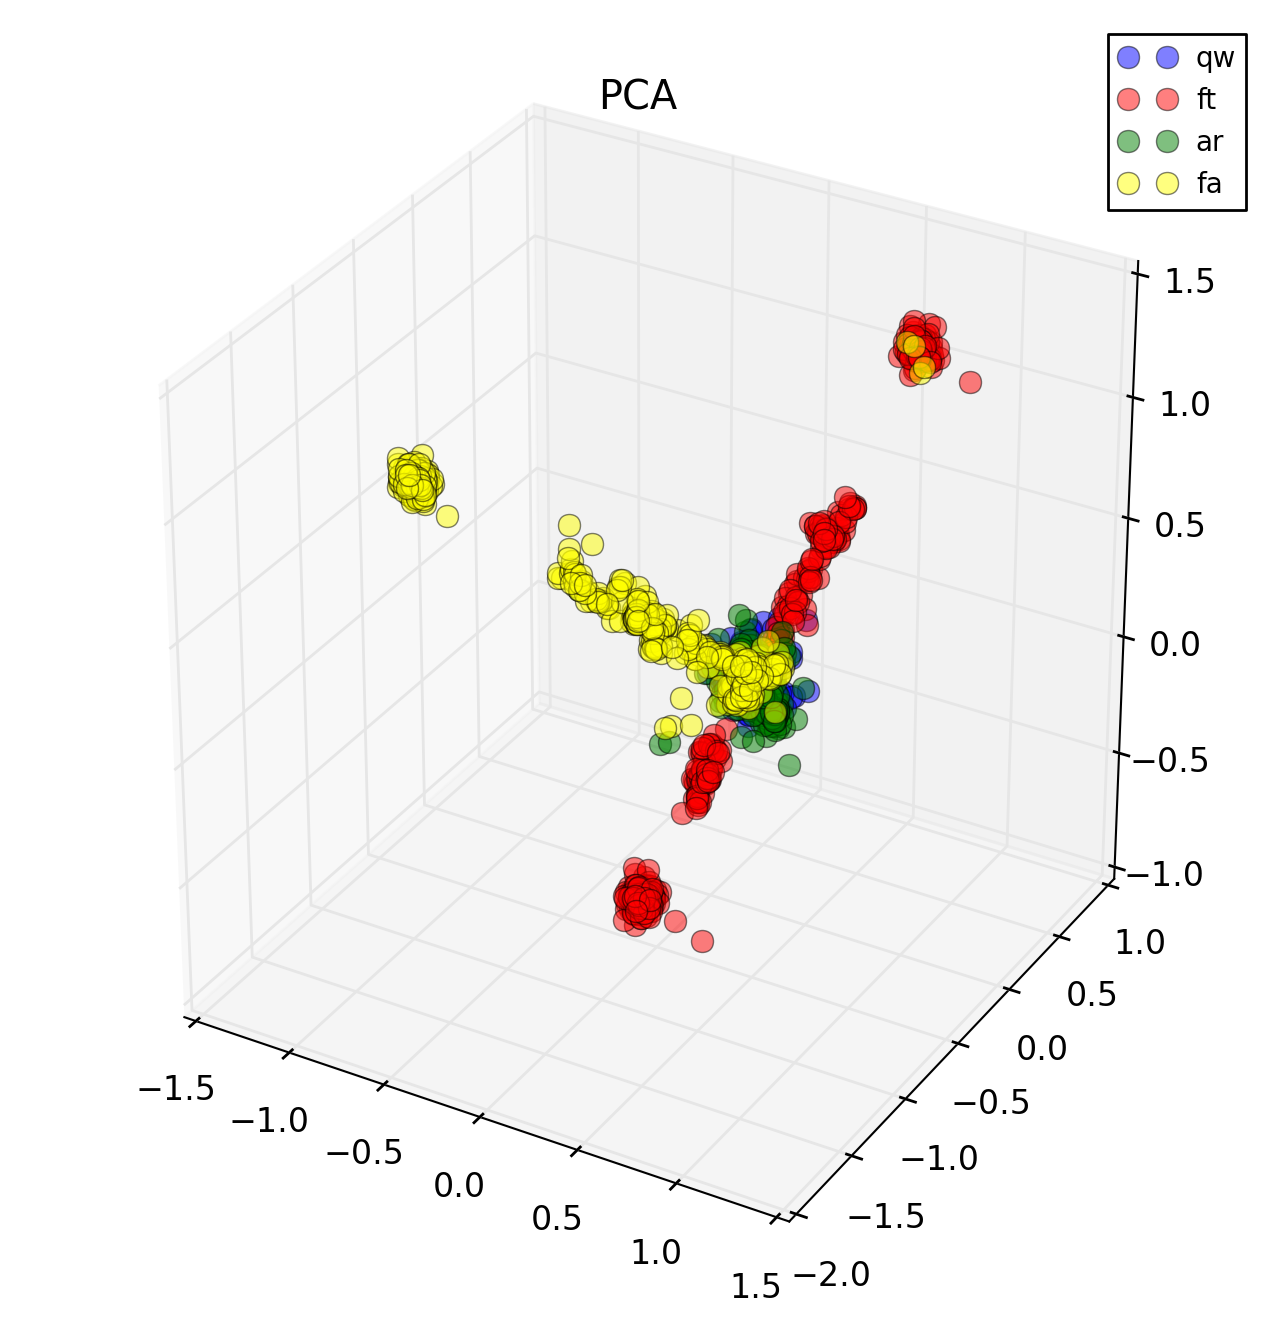
\includegraphics[width=1\textwidth]{img/easy_pca_3d}
\caption{3D PCA.}
\label{fig:3d_pca}
\end{minipage}
\end{figure}

Though, the classification task seems easy considering the previous tag examples, it gets more complicated when we handle other utterance choices. Figure~\ref{fig:2d_pca} and Figure~\ref{fig:3d_pca} show the scatter diagram after applying PCA to utterance embedding of the 5 most frequent tags (\emph{Statement-non-opinion}, \emph{Acknowledge}, \emph{Statement-opinion}, \emph{Accept}, \emph{Turn exit}), which account for $78\%$ of the corpus.

\begin{figure}
\centering
\begin{minipage}{.23\textwidth}
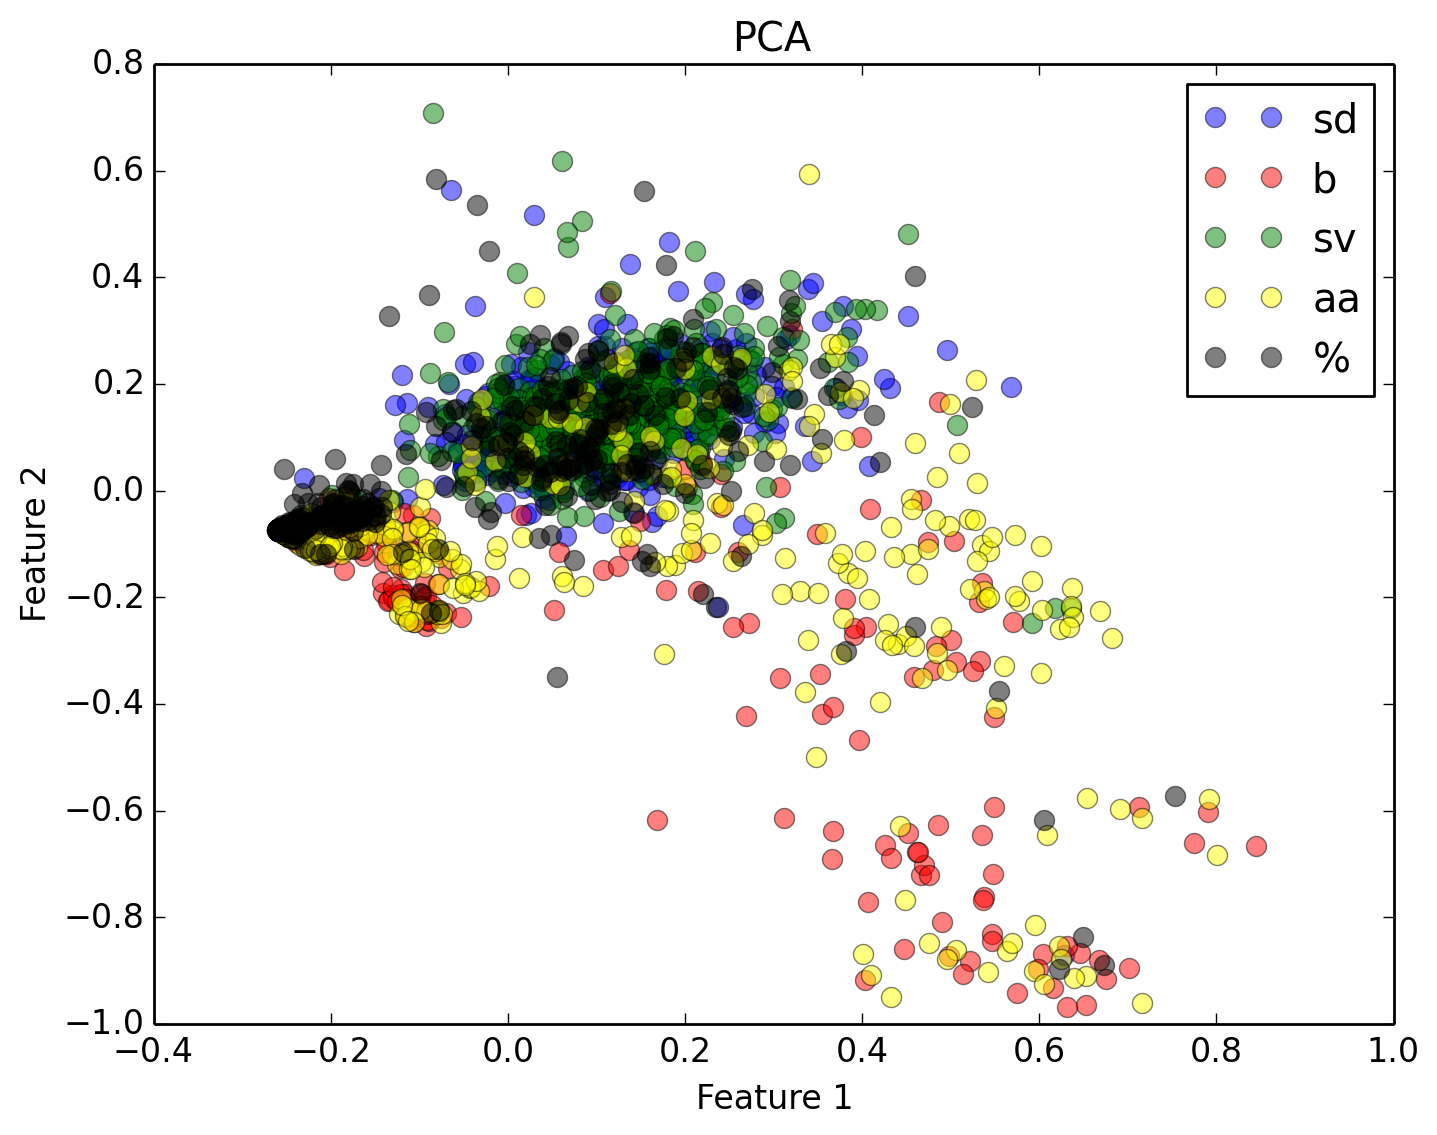
\includegraphics[width=1\textwidth]{img/complex_pca_2d}
\caption{2D PCA.}
\label{fig:2d_pca}
\end{minipage}
\begin{minipage}{.23\textwidth}
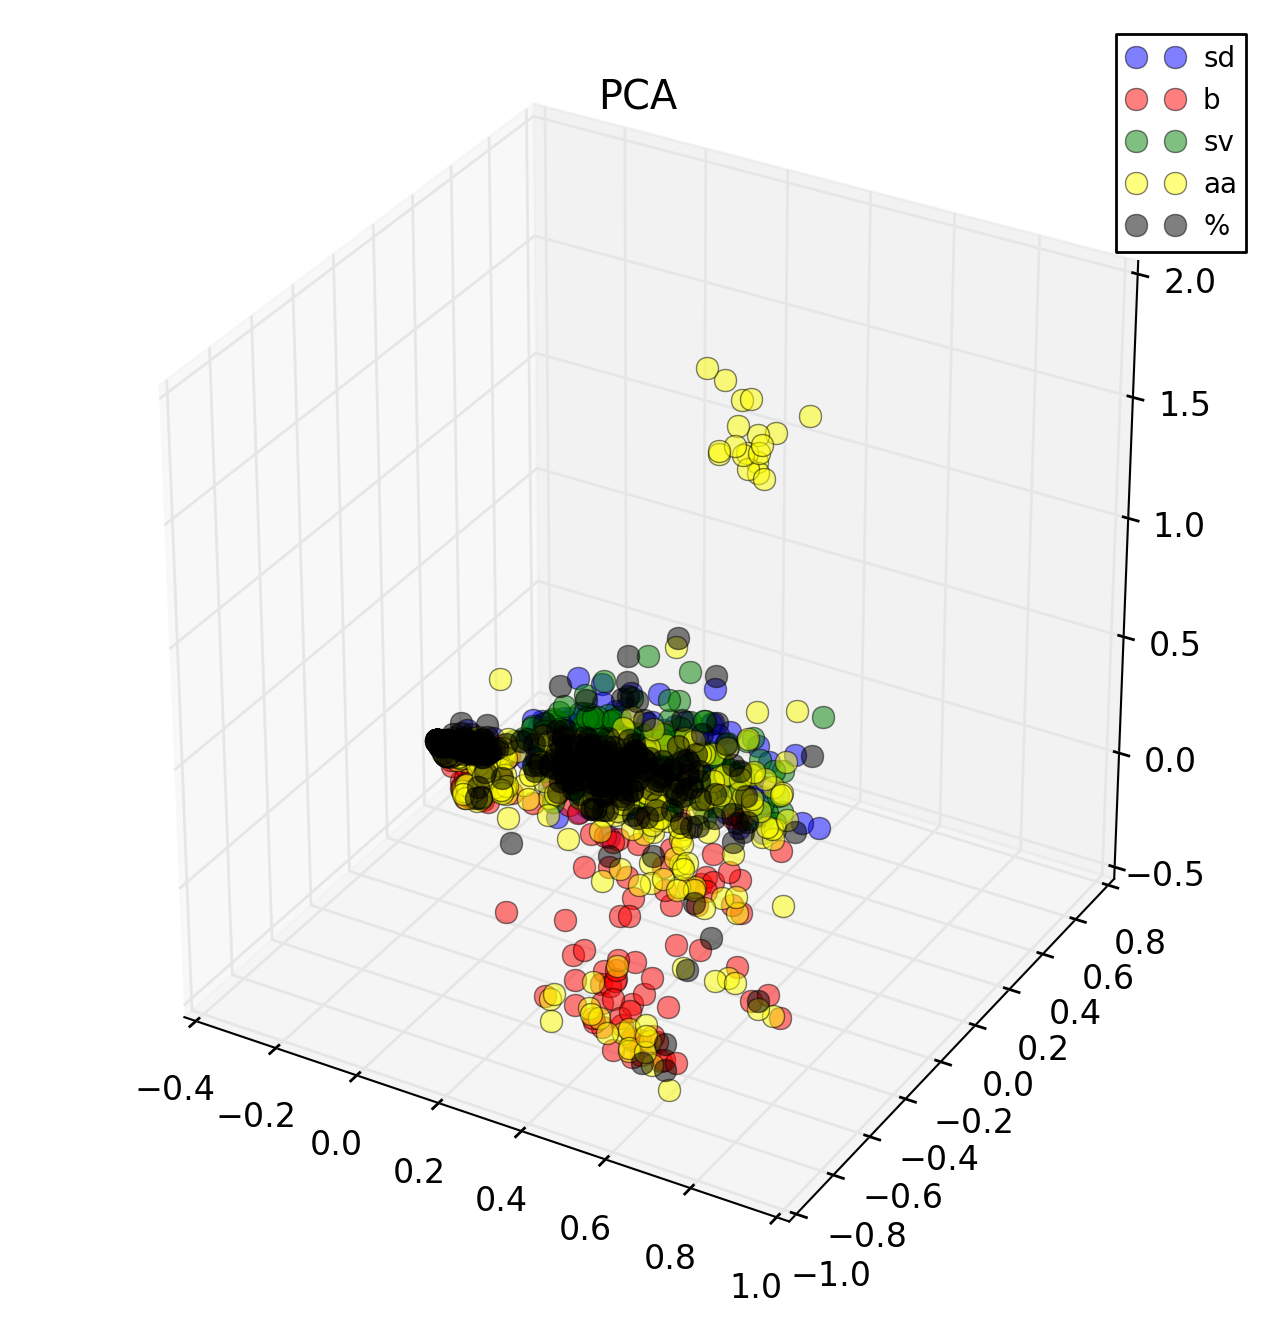
\includegraphics[width=1\textwidth]{img/complex_pca_3d}
\caption{3D PCA.}
\label{fig:3d_pca}
\end{minipage}
\end{figure}